\chapter{Communication Protocol}

This section describes the communication protocol used for command and data exchange between bus participants. Further, the bus monitor module, which is part of the \gls{FBU} is explained.

\section{Protocol}

In our approach a simple master-slave protocol was defined to enable communication between the master (\gls{ECU}, \gls{FBU}) and the slaves (\gls{THS}, \gls{MCU}, \gls{FBU}).
The protocol consists of command and data packets, each of them contains just one byte.
No error protection measures were taken into account.
Each bus participant needs a unique address. Since this design just contains three control units, two bits as address field are sufficient. Figure \ref{fig:Protocol} shows the composition of a control and data packets.

\begin{figure}[h!]
    \centering
    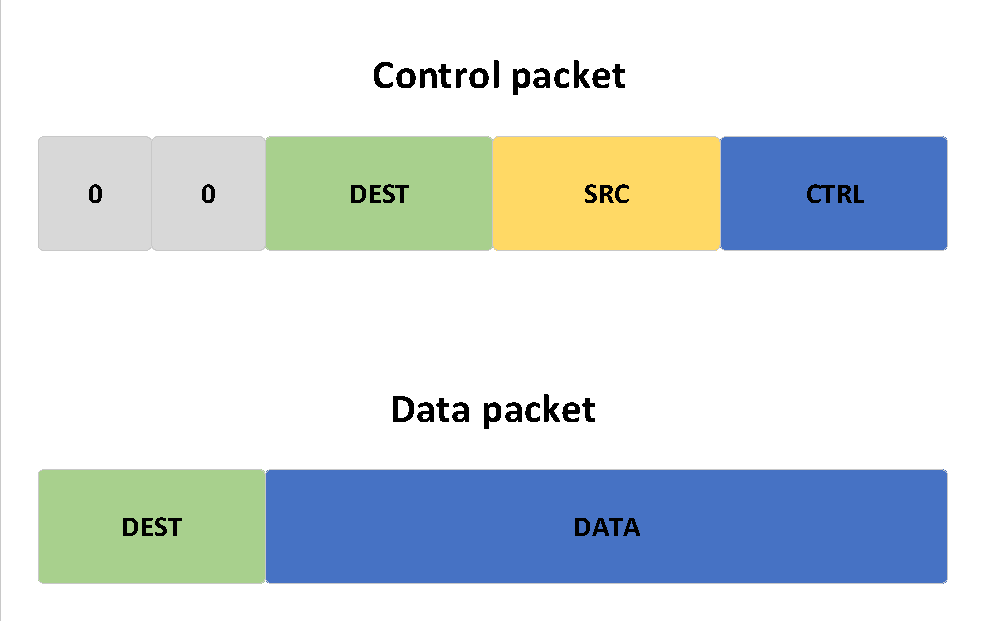
\includegraphics[width=0.75\textwidth]{figures/Protocol.pdf}
    \caption{Composition of control and data packets}\label{fig:Protocol}
\end{figure}

A control packet is indicated by two leading zeroes, followed by destination address (DEST) and source address (SRC). The last two bits (CTRL) determine a further classification of the control packet, as shown in table \ref{tab:controlPacket}.

\begin{table}[h!]
\begin{center}
\begin{tabular}{|c|c|c|}
\hline
\multicolumn{2}{|c|}{\textbf{CTRL}}&\textbf{Function} \\
\hline
0 & 0 & Request data \\
\hline
0 & 1 & Acknowledge \\
\hline
1 & 0 & Error 1 \\
\hline
1 & 1 & Error 2 \\
\hline
\end{tabular}
\label{tab:controlPacket}
\end{center}
\caption{Control packet classification}
\end{table}

A control packet can be used to request data, send an acknowledge or indicate errors. Only the master is able to send a request data command, the remaining control packet classifications can be used by the slaves, too.

A data packet starts with the destination address (DEST), followed by a 6 bit wide data field (DATA). It can be sent by the master and by slaves (if a request data command was received previously). If sent by a master, the slave has to answer with an acknowledge.

\section{Bus monitor}

The bus monitor module is part of the \gls{FBU} and is responsible for monitoring the traffic on the communication link to detect faulty units.

\begin{figure}[h!]
    \centering
    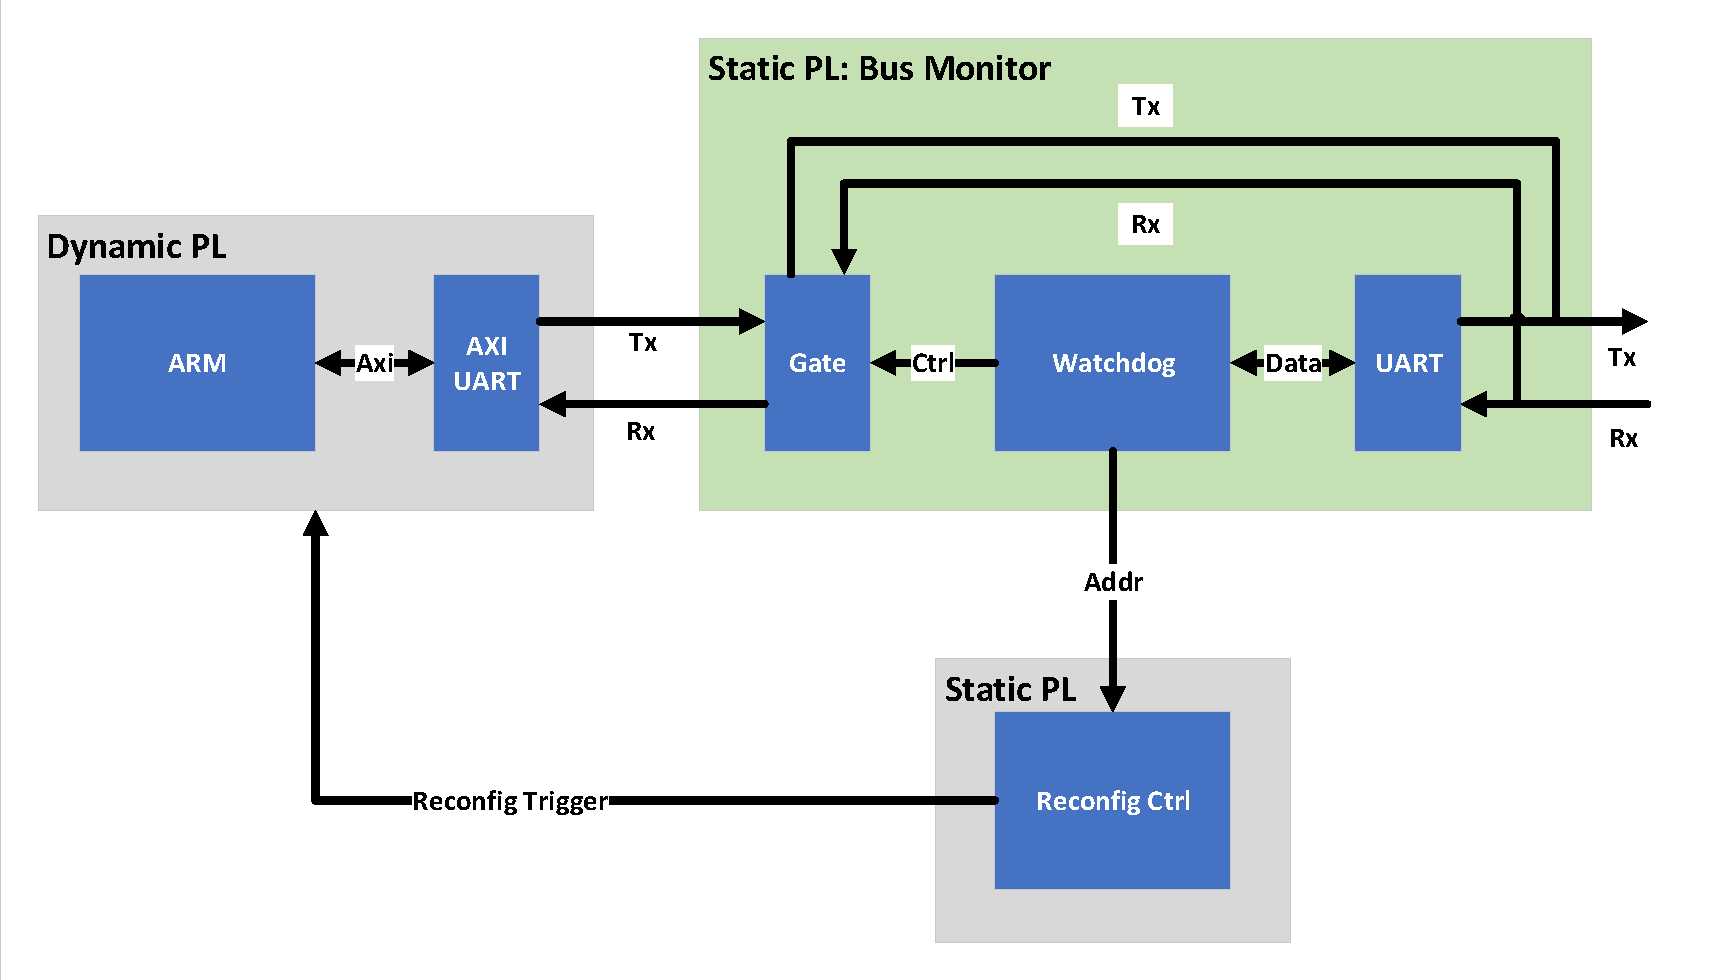
\includegraphics[width=\textwidth]{figures/BusMonitor.pdf}
    \caption{Bus monitor interfacing}\label{fig:BusMonitor}
\end{figure}
